\documentclass{article}
\usepackage{listings}
\usepackage{graphicx} % Required for inserting images
\usepackage{color}
\usepackage[a4paper, total={6.5in, 10in}]{geometry}
\usepackage{enumitem}

\lstnewenvironment{C}
  {\lstset{language=C}} 
%Add your addition parameters as required like showstringspaces , line numbering , 
% frames , etc.seperated by a comma as shown in the CPP  environment 
  {}
\lstnewenvironment{CPP}
  {\lstset{language=C++,basicstyle=\ttfamily\small,frame=none}}
  {}
\lstnewenvironment{Java}
  {\lstset{language=Java}}
  {}
\lstnewenvironment{Python}
  {\lstset{language=Python}}
  {}

% \title{\huge TP3 Report \\ Artificial Intelligence}
% \author{Bruno Luiz Dias Alves de Castro \\ Victor Gabriel Mendes Sündermann}
% \date{April 2023}

\begin{document}

\begin{titlepage}
\centering
{\textsc{\Large ESIEE Paris \\ ~\\ Artificial Intelligence and Cybersecurity} \par}
\vfill
{\huge\bfseries Artificial Intelligence \par}
\vspace{0.5cm}
{\LARGE Lab 3 Report \par}
\vspace{2cm}
{\Large\itshape Bruno Luiz Dias Alves de Castro \par}
{\Large\itshape Victor Gabriel Mendes Sündermann \par}
\vfill

% Bottom of the page
{\large \today\par}
\end{titlepage}

\pagebreak
\tableofcontents
\pagebreak

\section{Introduction}

In this report we will present the results of the fourth project of the Artificial Intelligence course. The project consists of implementing reinforcement learning algorithms and agents to score actions on a grid and eventually solve the \textbf{Pacman} game.
The topics worked on this lab were: Value Iteration, Q-Learning, and aproximate Q-Learning.

\section{Value Iteration}
To run the program, we use the following command:

\hbox{}

\definecolor{light-gray}{gray}{0.95}
\begin{lstlisting}[language=bash, frame=tlbr, framesep=6pt, backgroundcolor=\color{light-gray}]
  python3 gridworld.py -a value -i 5
\end{lstlisting}

\hbox{}

This test created the expected output as shown in the following image:

\hbox{}
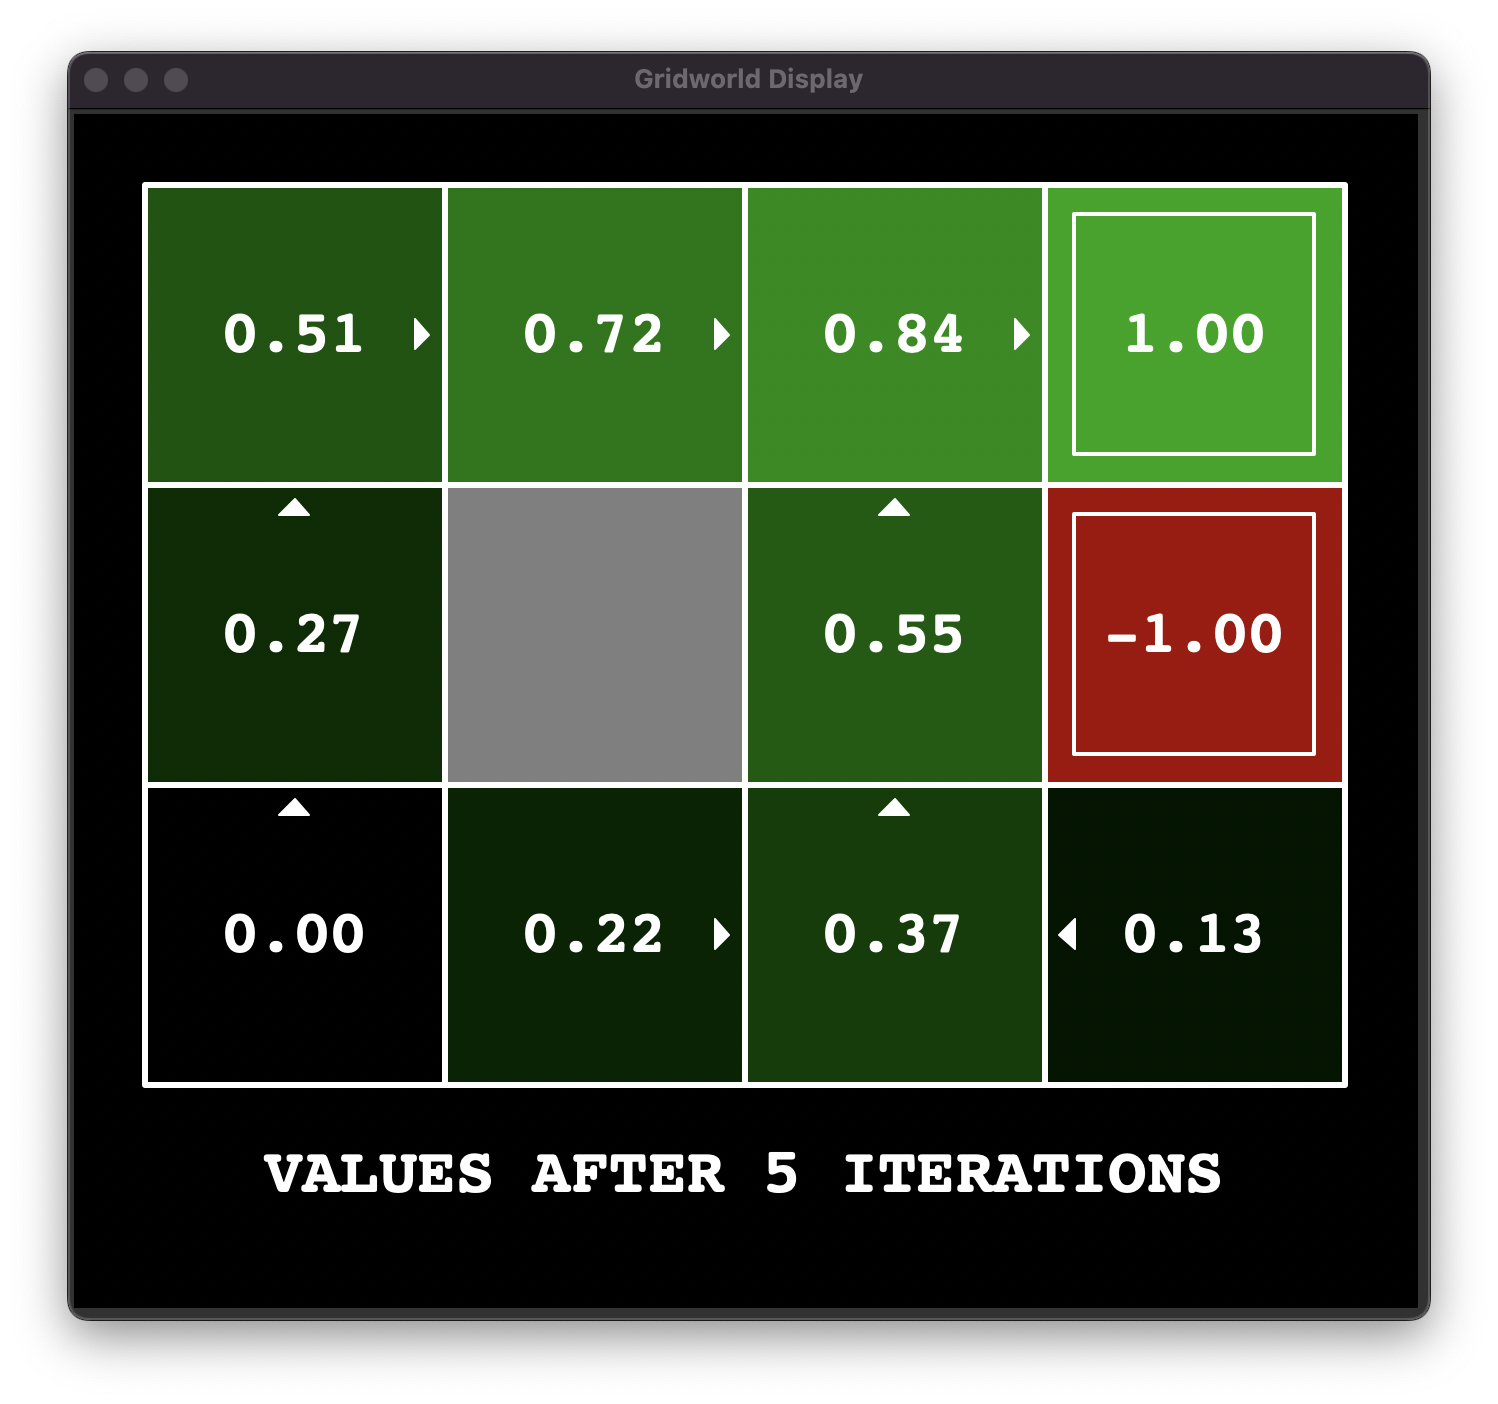
\includegraphics[width=0.5\textwidth]{images/gridWorld-ex2.png}
\hbox{}

\section{Q-Learning}

\hbox{}

\begin{lstlisting}[language=bash, frame=tlbr, framesep=6pt, backgroundcolor=\color{light-gray}]
    return score + closestFoodScore - closestGhostScore
\end{lstlisting}

\hbox{}

We also decided on using the Manhattan distance to calculate the distance between Pacman, the ghosts and the food pellets, because it is a less computationally expensive sollution to this problem, and don't really affect the final score.

\hbox{}

Finally, the result we got is the following:

\hbox{}

\begin{lstlisting}[language=python, frame=tlbr, framesep=6pt, backgroundcolor=\color{light-gray}]
def evaluationFunction(self, currentGameState, action):

    """ VARIABLES """

    foodList = newFood.asList()

    # manhattan distance
    foodDistances = \
        [manhattanDistance(newPos, food) for food in foodList]
    ghostDistances = \
        [manhattanDistance(newPos, ghost) for ghost in newGhostsPos]

    # closest food and ghost
    closestFood = min(foodDistances) if len(foodDistances) > 0 else 0
    closestGhost = min(ghostDistances) if len(ghostDistances) > 0 else 0

    # score calculation for food and ghost
    closestFoodScore = 0 if closestFood == 0 else 1.0/closestFood
    closestGhostScore = 0 if closestGhost == 0 else 1.0/closestGhost

    score = closestFoodScore - closestGhostScore

    return successorGameState.getScore() + score
\end{lstlisting}

\subsection{Tests}

In order to test our new evaluation function, we executed the following tests:

\subsubsection{testClassic}
\label{sec:testClassic}

\textbf Command:

\begin{lstlisting}[language=bash, frame=tlbr, framesep=6pt, backgroundcolor=\color{light-gray}]
    python3 pacman_AIC.py -p ReflexAgent -l testClassic
\end{lstlisting}

\noindent\textbf Output:

\begin{lstlisting}[language=bash, frame=tlbr, framesep=6pt, backgroundcolor=\color{light-gray}]
  Pacman emerges victorious! Score: 562
  Average Score: 562.0
  Scores:        562.0
  Win Rate:      1/1 (1.00)
  Record:        Win
\end{lstlisting}

\subsubsection{mediumClassic}
\label{sec:mediumClassic}

- One ghost test run \\
~\\
\textbf Command:

\begin{lstlisting}[language=bash, frame=tlbr, framesep=6pt, backgroundcolor=\color{light-gray}]
    python3 pacman_AIC.py -p ReflexAgent -k 1
\end{lstlisting}

\noindent\textbf Output:

\begin{lstlisting}[language=bash, frame=tlbr, framesep=6pt, backgroundcolor=\color{light-gray}]
    Pacman emerges victorious! Score: 1485
    Average Score: 1485.0
    Scores:        1485.0
    Win Rate:      1/1 (1.00)
    Record:        Win
\end{lstlisting}

~\\
- Two ghosts test run \\
~\\
\textbf Command:

\begin{lstlisting}[language=bash, frame=tlbr, framesep=6pt, backgroundcolor=\color{light-gray}]
    python3 pacman_AIC.py -p ReflexAgent -k 2
\end{lstlisting}

\noindent\textbf Output:

\begin{lstlisting}[language=bash, frame=tlbr, framesep=6pt, backgroundcolor=\color{light-gray}]
    Pacman emerges victorious! Score: 1407
    Average Score: 1407.0
    Scores:        1407.0
    Win Rate:      1/1 (1.00)
    Record:        Win
\end{lstlisting}

\subsubsection{No layout 20 runs average}
\label{sec:20runs}

During this part of the testing, we ran the \textbf{ReflexAgent} 20 times on each of the 6 conbinations of the settings listed below, and calculated the average score and the win rate. The possible settings are as listed (indentified with the letters a-e):

\begin{itemize}
  \item Possible settings:
  \begin{enumerate}[label=(\alph*)]
    \item One ghost
    \item Two ghosts
    \item Random ghosts
    \item Random ghosts with fixed seed
    \item Non random ghost
  \end{enumerate}
\end{itemize}

~\\
The results obteined are shown in Table \ref{tab:reflexagent}.

\begin{table}[!ht]
  \begin{center}
  \begin{tabular}{||c||c|c|c|c|c|c||}
  \hline
  Configuration & (a, c) & (a, d) & (a, e) & (b, c) & (b, d) & (b, e) \\
  \hline\hline
  Average Score & 671.65 & 785.2 & 449.9 & 464.7 & 228.7 & -14.25 \\
  \hline\hline
  Win Rate & 14/20 (0.70) & 18/20 (0.90) & 10/20 (0.50) & 10/20 (0.50) & 6/20 (0.30) & 1/20 (0.05) \\
  \hline
  \end{tabular}
  \caption{ReflexAgent test results}
  \label{tab:reflexagent}
  \end{center}
\end{table}

\subsubsection{Results}
The \textbf{ReflexAgent} was sucessful in clearing most of the purposed tests. Especially the the ran in sections \ref{sec:testClassic} and \ref{sec:mediumClassic} (\textbf{testClassic} and \textbf{mediumClassic}), were no problem for the agent.

Things start to fall short when it comes to test in section \ref{sec:20runs}. The agent obtained decent success in the test with a single ghost, but performenced declined on tests with two ghost. The agent only cleared 6 out of 20 tests with random ghosts, and was onle able to clear a single test with non random ghosts.

\hfill\break
\pagebreak
\section{Minimax algorithm}

The Minimax algorithm consists in the following idea: two "players" (or agents) are competing against each other in a game. As both players equally want to win this game, if we assume the point of view of one of them, we can say that player wish to maximize its score, and the opponent is trying to maximize the most it can.

It's possible to simulate such a scenario, by making both players take turns, and attributing a "score" to each play. Every time a "maximizer player" plays, it chooses the maximum score possible, and every time a "minimizer" player player, it chooses the minimum score available.

By simulate all possible plays in a game from a given game state, we can write an algorithm that alternate between maximize and minimize plays, and chooses the optimal path in a tree of possible outcomes for the game. This takes into account that all players always take the best play possible (what may not happen in all scenarios, we explore this further in Section~\ref{sec:expectimax}).
~\\
~\\
An implementation of such approch is described in the following section.

\subsection{Minimax implementation}

To make this implementation possible, we started by implementing two functions: one for the maximizer (Pacman), and one for the minimizer (ghosts). We start by calling the maximizer, that looks for all possible plays of the minimizer agent. They recursivly call each other, until a "depth" parameters reachs zero, or the game terminates. This depth parameter is necessary, because of the complexity of this algorithm. As every agent calls the next on recursivly, this results in a tree of calls that expands indefinetly until the end of the game is reach. If we don't interupt the search, this algorithm would take ages to compute a play.
~\\
~\\
The implementation of both functions can be seen in Tables~\ref{tab:minimax-maximizer} and~\ref{tab:minimax-minimizer}.

\begin{table}[!ht]
\begin{lstlisting}[language=python, frame=tlbr, framesep=6pt, backgroundcolor=\color{light-gray}]
def MAX_VALUE(self, gameState, d):
    if d == 0 or gameState.isWin() or gameState.isLose():
        # base case: return evaluation function
        return self.evaluationFunction(gameState), Directions.STOP
    
    bestScore, bestAction = -math.inf, Directions.STOP

    for action in gameState.getLegalActions(0):
        successors = gameState.generateSuccessor(0, action)

        # call minimaxer agent (ghosts)
        value, _ = self.MIN_VALUE(successors, d, 1)

        # update best score and action
        if value > bestScore:
            bestScore, bestAction = value, action

    return bestScore, bestAction
  \end{lstlisting}
  \caption{Maximizer function}
  \label{tab:minimax-maximizer}
\end{table}

\begin{table}[!ht]
\begin{lstlisting}[language=python, frame=tlbr, framesep=6pt, backgroundcolor=\color{light-gray}]
def MIN_VALUE(self, gameState, d, indexAgent):
    if d == 0 or gameState.isWin() or gameState.isLose():
        # base case: return evaluation function
        return self.evaluationFunction(gameState), Directions.STOP

    bestScore, bestAction = math.inf, Directions.STOP

    for action in gameState.getLegalActions(indexAgent):
        successors = gameState.generateSuccessor(indexAgent, action)
        if indexAgent == gameState.getNumAgents() - 1:
            # call pacman
            value, _ = self.MAX_VALUE(successors, d - 1)
        else:
            # call next ghost
            value, _ = self.MIN_VALUE(successors, d, indexAgent + 1)

        # update best score and action
        if value < bestScore:
            bestScore, bestAction = value, action

    return bestScore, bestAction
\end{lstlisting}
\caption{Minimizer function}
\label{tab:minimax-minimizer}
\end{table}

In the case of the minimizer function, when calculating the possible plays for it's children, it first call the remaining ghosts. If all ghosts already played that turn, it then calls the maximizer (Pacman), and decreases the depth parameter.

\subsection{Tests}

In order to test the Minimax algorithm implemented, we ran it 20 times, using different depths, and the results are shown in the table below: \\

\begin{table}[ht]
  \begin{center}
  \begin{tabular}{||c||c|c|c||}
    \hline
    Depth & 2 & 3 & 4 \\
    % \hline\hline
    % Iteration & - & - & - \\
    % \hline
    % 1 & -231 (L) & -276 (L) &  840 (W) \\
    % \hline
    % 2 & -206 (L) & 1254 (W) &   32 (L) \\
    % \hline
    % 3 & -244 (L) & -336 (L) & 1732 (W) \\
    % \hline
    % 4 & -154 (L) & -263 (L) & -314 (L) \\
    % \hline
    % 5 & 1249 (W) &  966 (W) &  311 (W) \\
    % \hline
    % 6 & -688 (L) &  -96 (L) &  540 (L) \\
    % \hline
    % 7 & -185 (L) & 1138 (W) &  204 (L) \\
    % \hline
    % 8 & -203 (L) &  959 (W) &  479 (L) \\
    % \hline
    % 9 & -239 (L) & 1531 (W) & 1171 (W) \\
    % \hline
    % 10 & -140 (L) &  116 (L) &  -97 (L) \\
    % \hline
    % 11 & -317 (L) & 1373 (W) &  896 (W) \\
    % \hline
    % 12 &  178 (L) & 1039 (W) & 1218 (W) \\
    % \hline
    % 13 & -176 (L) & -174 (L) & 1048 (W) \\
    % \hline
    % 14 & -624 (L) & 1168 (W) &  223 (L) \\
    % \hline
    % 15 & -180 (L) & -156 (L) &  402 (L) \\
    % \hline
    % 16 & -238 (L) &  749 (W) & 1238 (W) \\
    % \hline
    % 17 & -243 (L) & -267 (L) & 1202 (W) \\
    % \hline
    % 18 &    8 (L) & 1147 (W) & 1631 (W) \\
    % \hline
    % 19 & -368 (L) & 1319 (W) &  277 (L) \\
    % \hline
    % 20 & -454 (L) & -272 (L) &  985 (W) \\
    \hline\hline
    Average &  -173 &  546 &  701 \\
    \hline\hline
    Best & 1249 & 1531 & 1732 \\
    \hline\hline
    Win Rate & 1/20 (0.05) & 11/20 (0.55) & 11/20 (0.55) \\
    \hline
  \end{tabular}
  \caption{Minimax test results}
  \label{tab:minimax}
  \end{center}
\end{table}

Analysing the results, we reached the following conclusions: First, is that the algorithm performs better the more depth we add to the search. This is no surprise: the more we search the tree, the closer we approch the optimal sollution.
Lastly, the more we increment the depth, the more time it takes to conclude the search. Due to the exponential nature of this algorithm, it's not possible to go much further than what we already done. With a depth of 4 it already took close to an hour to terminate. Luckly, there is an improvement that can be done to acelerate this process a bit, and we explore it in the next section.

\pagebreak
\section{AlphaBeta algorithm}

The Alpha Beta implementation for the Minimax algorithm consists of two main changes: the addition of two parameters, alpha and beta, and the pruning of the search tree.

The parameters alpha and beta helps the algorithm identify if it is possible to continue searching the tree, or if a optimal value was already reached. In this case, we proceed with the pruning of the search tree, and return the value of the node.

This pruning is done in both the minimizer and maximizer functions, and help us reduce the number of nodes that are evaluated, and therefore, the time it takes to find the optimal move. This translates into a considerable performance improvement, as we will see in the next section.

\subsection{AlphaBeta implementation}

In order to implement the AlphaBeta algorithm, we used the same functions as the Minimax algorithm, but added two parameters to the functions, alpha and beta. The alpha and beta parameters are used to prune the search tree, and are initialized as \textbf{-math.inf} and \textbf{math.inf} respectively. The alpha and beta parameters are updated in the minimizer function, and the maximizer function, as shown in the code below:

\begin{table}[!ht]
  \begin{lstlisting}[language=python, frame=tlbr, framesep=6pt, backgroundcolor=\color{light-gray}]
    """ CODE """

    if value > beta:
      return value, action

    alpha = max(alpha, value)

    """ CODE """
  \end{lstlisting}
  \caption{Maximizer function with beta pruning}
\end{table}

\begin{table}[!ht]
  \begin{lstlisting}[language=python, frame=tlbr, framesep=6pt, backgroundcolor=\color{light-gray}]
    """ CODE """

    if value < alpha:
      return value, action

    """ CODE """
  \end{lstlisting}
  \caption{Minimizer function with alpha pruning}
\end{table}

\subsection{Tests}

In order to test the performance of the Alpha Beta algorithm, we used the same tests as the Minimax algorithm, and compared the results. The results are shown in the table below:

~\\
\begin{table}[!ht]
  \begin{center}
    \begin{tabular}{||c||c|c|c|c||}
      \hline
      Depth & 2 & 3 & 4 \\
      \hline\hline
      Average &  -121.5 &  413.6 &  635.85 \\
      \hline\hline
      Best & 1001 & 1604 & 1701 \\
      \hline\hline
      Win Rate & 1/20 (0.05) & 9/20 (0.45) & 11/20 (0.55) \\
      \hline
    \end{tabular}
    \caption{AlphaBeta test results}
    \label{tab:alphabeta}
  \end{center}
\end{table}

\subsubsection{Performance comparison with Minimax}
After running the tests, we compared the performance of the Minimax (Table~\ref{tab:minimax}) and Alpha Beta (Table~\ref{tab:alphabeta}) algorithms.

As expected, the performance between the two algorithms is pratically the same. That's expected, as the main functionallity of both algorithm is the same, the onlt different between the two being the pruning in the Alpha Beta version.

Where the difference is definitely noticeable is in the runtime of both algorithms. To test this, we ran the same tests as before, but with a depth of 3, and compared the results. The results are shown in Table~\ref{tab:minimax_vs_alphabeta}. As we can see, the Alpha Beta algorithm is 15.6\% faster than the Minimax algorithm.

~\\
\begin{table}[!ht]
  \begin{center}
    \begin{tabular}{||c||c|c|c||}
      \hline
      Algorithm & Minimax & AlphaBeta \\
      \hline\hline
      Time & 167.78s & 145.10s \\
      \hline\hline
      Speedup & - & 15.6\% \\
      \hline
    \end{tabular}
    \caption{Minimax VS AlphaBeta (Depth=3)}
    \label{tab:minimax_vs_alphabeta}
  \end{center}
\end{table}

The speedup obtain in this test is not that significant, but it is still a considerable improvement. This shy performance improvement is most likely due to the fact that the main botleneck of the algorithm is not the search. In our tests, we noticed that, due to the depth limit, when the Pacman eventually gets isolated in a area of the maze with no food, the algorithm doesn't really know what to do, and this leads to games that take a long time to finish.

To verify this, we ran the same test with the DirectinalGhost option. This forces the Pacman to move more frequently (as it is now being more effectively chased by the ghosts), but due to the exploration depth limitation, it loses games more oftenly. The results are shown in Table~\ref{tab:minimax_vs_alphabeta2}.

Now the speedup is much more significant, as the Alpha Beta algorithm is 83.5\% faster than the Minimax algorithm. There is still more room to improvement though, but the performance gain is already considerable.

~\\
\begin{table}[!ht]
  \begin{center}
    \begin{tabular}{||c||c|c|c||}
      \hline
      Algorithm & Minimax & AlphaBeta \\
      \hline\hline
      Time & 38.58s & 21.03s \\
      \hline\hline
      Speedup & - & 83.5\% \\
      \hline
    \end{tabular}
    \caption{Minimax VS AlphaBeta (Depth=3, DirectionalGhost)}
    \label{tab:minimax_vs_alphabeta2}
  \end{center}
\end{table}

\pagebreak
\section{Expectimax algorithm}

The Expectimax algorithm is a varation of the Minimax algorithm. In this version, the minimizer function is replaced by an expectation function, which calculates the expected value of the next move. This is done by calculating the average of the values of all the possible moves.

This is extremelly usefull in our Pacman case, especially in cases where we execute the simulations with a random ghost movement. In these scenarios, the minimizer is as likely to take the worst movement possible as it is to do the best. The clasical algorith is great when the movements are always the best ones, but starts to fall apart when the opponent makes unexpected decisions. Knowing this, we alter the minimizer function to calculate an expected value instead of the absolute best one (the minimum in this case).

We describe the implementation in the next section.

\subsection{Expectimax implementation}
\label{sec:expectimax}

In order to implement the Expectimax algorith, the only change necessary is done to the Minimizer function. We used the same one implementd before, and added the following code to it:

\begin{table}[!ht]
  \begin{lstlisting}[language=python, frame=tlbr, framesep=6pt, backgroundcolor=\color{light-gray}]
    def MIN_VALUE(self, gameState, d, indexAgent, alpha, beta):
      """ CODE """

      value = value / len(gameState.getLegalActions(indexAgent))
      bestScore += value

      """ CODE """
  \end{lstlisting}
  \caption{Expectimax implementation}
\end{table}

\subsection{Expectimax tests}

We ran the same tests as before, but with the Expectimax algorithm. The results are shown in Table~\ref{tab:expectimax}.

~\\
\begin{table}[!ht]
  \begin{center}
    \begin{tabular}{||c||c|c|c|c||}
      \hline
      Depth & 2 & 3 & 4 \\
      \hline\hline
      Average & 97.85 & 551.3 & 873.15 \\
      \hline\hline
      Best & 1031 & 1397 & 1515 \\
      \hline\hline
      Win Rate & 4/20 (0.20) & 10/20 (0.50) & 15/20 (0.75) \\
      \hline
    \end{tabular}
    \caption{Expectimax test results}
    \label{tab:expectimax}
  \end{center}
\end{table}

\pagebreak
\section{Bonus: Evaluation function improvement}

After implementing and running countless test to all algorithm proposed, we identified a serious problem with the evaluation function used in the project: It was the main piece holding our implementations back, and the perormance of our algorithms were suffering a lot because of it.

The default evaluation function implemented in the project is the \textit{\textbf{scoreEvaluationFunction}}. The evaluation function only takes into account the current score of the games. It gets the work done in some of the cases, but has two serious draw-backs: It doesn't take into account the number of food left in the maze, and it doesn't take into account the distance to the closest food. As a result, when the Pacman gets "isolated" in a part of the map without any food, it hasn't anything to maximize, and needs a ghost to approch in order to proceed the game.

To solve this problem, we sugest a new evaluation function, called \textit{\textbf{betterEvaluationFunction}}. It's implementation and functionallity is explained in the following section.

\subsection{The new evaluation function: betterEvaluationFunction}

The proposed evaluation function takes into account this two extra parameters (along with the score): \textit{the number of food pallets left} and \textit{the distance to the closest food}. The number of food pallets left encourages the Pacman to eat more pallets when stuck, and the distance to the closest food will prevent the Pacman of isolating itself in the maze.

the implementation is described in the following section.

\subsubsection{betterEvaluationFunction implementation}

To implement the new evaluation function, we created a new function in the code, as follows:

\begin{table}[!ht]
  \begin{lstlisting}[language=python, frame=tlbr, framesep=6pt, backgroundcolor=\color{light-gray}]
def betterEvaluationFunction(currentGameState):
  """
  Your extreme ghost-hunting, pellet-nabbing, food-gobbling, unstoppable
  evaluation function (question 8).

  DESCRIPTION: <write something here so we know what you did>
  """
  
  def closestFoodDistance(gameState):
    pacmanPosition = gameState.getPacmanPosition()
    foodList = gameState.getFood().asList()

    if len(foodList) == 0:
        return 0

    return min([manhattanDistance(pacmanPosition, food) for food in foodList])

  closestFood = closestFoodDistance(currentGameState)
  return currentGameState.getScore() - (10 * closestFood) \ 
    - (100 * currentGameState.getNumFood())
  \end{lstlisting}
  \caption{betterEvaluationFunction implementation}
\end{table}

For calculation the distance to the closest food, we used the the Manhattan Distance (implemented in the function itself), and the number of food is retrieved from the game state. They are multiplied by 10 and 100, respectively, in order to have a bigger impact in the final score, and subtracted from the current game score.

The results of our implementation is showed in the next section.

\subsubsection{betterEvaluationFunction tests}

To test the new \textit\textbf{{betterEvaluationFunction}}, we repeated the same tests executed before, now using the this new evaluation function instead of the old \textit\textbf{{scoreEvaluationFunction}}. We chose the  \textit\textbf{{Expectimax agent}} to run the tests. Its description and implementation can be found in Section~\ref{sec:expectimax}.
~\\
~\\
The result of the tests can be found in Table~\ref{tab:expectimax-better}.

~\\
\begin{table}[!ht]
  \begin{center}
    \begin{tabular}{||c||c|c|c|c||}
      \hline
      Depth & 2 & 3 & 4 \\
      \hline\hline
      Average &  1228.6 &  1340.15 &  1131.25 \\
      \hline\hline
      Best & 1724 & 1757 & 1743 \\
      \hline\hline
      Win Rate & 19/20 (0.95) & 20/20 (1.00) & 19/20 (0.95) \\
      \hline
    \end{tabular}
    \caption{Expectimax test results with betterEvaluationFunction}
    \label{tab:expectimax-better}
  \end{center}
\end{table}

Comparing both results of Tables~\ref{tab:expectimax} and~\ref{tab:expectimax-better}, it's possible to observe a huge gain in performance. By only altering the evaluation function, we were able to obtain way batter results, even reaching a Win Rate of 100\% in some test cases, and performing well in the cases with lower depths.

\pagebreak
\section{Conclusion}

\end{document}